\documentclass[a4paper,12pt]{article}
\usepackage[a4paper,top=1.5cm,left=2.1cm,right=2.1cm,bottom=1.8cm,includehead,includefoot]{geometry}
\usepackage[T1]{fontenc}
\usepackage[utf8]{inputenc}
\usepackage[english,bulgarian]{babel}
\usepackage{amssymb,amsmath, oz, mathrsfs}
\usepackage{url}
\usepackage{graphicx}
\usepackage{color,colortbl}
\usepackage{float}
 
\newtheorem{thm}{Теорема}[section]
\newtheorem{stm}{Твърдение}[section]
\newtheorem{lemma}{Лема}[section]
\newtheorem{defn}{Дефиниция}[section]
\newtheorem{example}{Пример}[section]
\newenvironment{mproof}{\paragraph{Доказателство}}{\hfill$\square$}

\DeclareMathOperator*{\argmax}{arg\,max}

\makeatletter
\newcommand{\xRightarrow}[2][]{\ext@arrow 0359\Rightarrowfill@{#1}{#2}}
\newcommand{\dslash}{\slash\slash}
\makeatother

\begin{document}
\thispagestyle{empty}
\noindent\begin{minipage}{0.3\textwidth}

\includegraphics[width=10mm,scale=0.5]{figures/logo.jpg}
\end{minipage}%
\hfill%
\begin{minipage}{0.6\textwidth}\raggedleft
Катедра Математическа логика и приложения\\
Факултет по Математика и Информатика\\
Софийски Университет\\
\end{minipage}
\noindent\makebox[\linewidth]{\rule{\textwidth}{1pt}} 
\begin{center}
\begin{minipage}{0.75\linewidth}
    \centering
    \vspace{3cm}
    {\Large \textbf{Заглавие на дипломната работа на много редове}}\par
    \vspace{3cm}
    Дипломна работа\\ на\\ Нели Велиславова Хатева\\ студент специалност Информатика\\ ФН М29245\par
    \vspace{3cm}
    Ръководител \\доц. д-р Стоян Михов\par
    \vspace{3cm}
    2017 \par
    \vspace{3cm}
\end{minipage}
\end{center}
\clearpage

\tableofcontents
\listoffigures
\listoftables
\clearpage

\section{Увод}

  $\hspace*{1mm}$ В компютърните науки компресирането представлява кодиране на данни с цел намаляване на обема им.
  Данните могат да представляват както звуци и изображения, така и текст. Компресирането може да бъде с или без загуба на информация.
  При компресиране без загуба на информация оригиналните данни могат да бъдат възстановени изцяло, докато
  при компресиране със загуба на информация декомпресираните данни се отличават от оригиналните.
  Възниква и въпросът за компресиране на речник от думи на даден естествен език.

  $\hspace*{1mm}$ Всеки речник от думи на даден естествен език е краен списък, който може да се представи с математическия апарат на крайните автомати.
  Това представяне е широко използвано заради компактността му и множеството алгоритми за работа с него. Въпреки това, в много статии
  \cite{citation01, citation02, citation03, citation04} се разглеждат различни формализми, които компресират паметта за това представяне.
  Общото при тези подходи е, че езикът на изходния автомат не се променя, тоест компресирането е без загуба на информация.
  Фокусът на тази дипломна работа е компресията на естествен език със загуба на информация, като се изследва зависимостта между размера на паметта и различията в оригиналния
  и новополучения език.
  
\pagebreak

\section{Мотиви и интуиция}
  $\hspace*{1mm}$ Естествените езици подлежат на различни класификации спрямо набор от различни критерии. Една възможна класификация на езиците е морфологичната и
  типологичната класификация. Тя представлява групиране на езиците въз основа на граматичните отношения. Спрямо тази класификация има четири групи езици:
  инкорпориращи (полисинтетични), изолиращи (коренни), аглутиниращи и флективни. На практика повечето езици проявяват характеристики от различните групи и не могат
  еднозначно да се класифицират, но като цяло всички индоевропейски езици попадат в графата на флективните езици. За тях характерно е, че основното значение
  на думата се носи от нейния корен, а за изразяване на граматичнате категории се използват разнообразни флективни елементи.
  Забелязват се отпределени правила при употребата на флексиите, както и излючения от тези правила.
  Такива изключения възникват поради фонетични особености при произношение на думите, поради исторически причини и ред други.
  За пример в английския език множественото число на повчето думи се образува като към формата за единствено число прибавим \textbf{\emph{s}} на края.
  Но има думи, които са изключение от това правило. Например множественото число на думите,
  завършващи на \textbf{\emph{y}}, предшествано от съгласна, в единствено число, се образува като от основната форма премахнем \textbf{\emph{y}} и
  добавим \textbf{\emph{ies}}. Други пример за изключения при озбразуването на множествено число в английския език са двойките
  \textbf{\emph{foot}} - \textbf{\emph{feet}}, \textbf{\emph{person}} - \textbf{\emph{people}}. Примери в българския език за изключения са думи с така наречените
  променливо \textbf{\emph{я}} (\textbf{\emph{бял}} - \textbf{\emph{бели}}) и подвижно \textbf{\emph{ъ}} (\textbf{\emph{връх}} – \textbf{\emph{върхове}}).
  Универсален пример за изключения от правилото са думи, които имат форма само за единствено число (singulare tantum) или само за множествено число (plurale tantum).
  Примери за плуралия тантум в българския език са думите \textbf{\emph{трици}}, \textbf{\emph{въглища}}, \textbf{\emph{финанси}}, \textbf{\emph{очила}},
  \textbf{\emph{дънки}}, \textbf{\emph{джинси}}, а за сингулария тантум - \textbf{\emph{нефт}}, \textbf{\emph{захар}}, \textbf{\emph{ориз}}, \textbf{\emph{мас}},
  \textbf{\emph{желязо}} \cite{citation05}.

  Такива словоформи водят до увеличаване на размера на автомата, с който представяме езика.
  Ако премахнем словоформите, които са изключения от правилата за спрежение, и ги заменим със словоформи, образувани по правилата,
  тогава паметта за представянето на автомата ще бъде по-малка.
  Това се вижда лесно от следния пример:

\begin{figure}[H]
  \centering
  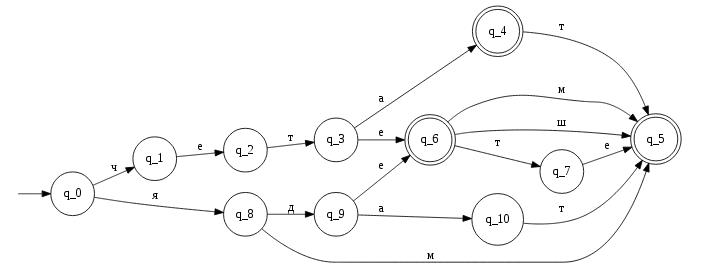
\includegraphics{figures/example1.jpg}
  \caption{Автомат, разпознаващ словоформите \textbf{\emph{ям}}, \textbf{\emph{ядеш}}, \textbf{\emph{яде}},
  \textbf{\emph{ядем}}, \textbf{\emph{ядете}}, \textbf{\emph{ядат}},
  \textbf{\emph{чета}}, \textbf{\emph{четеш}}, \textbf{\emph{чете}},
  \textbf{\emph{четем}}, \textbf{\emph{четете}}, \textbf{\emph{четат}}}
\end{figure}

\begin{figure}[H]
  \centering
  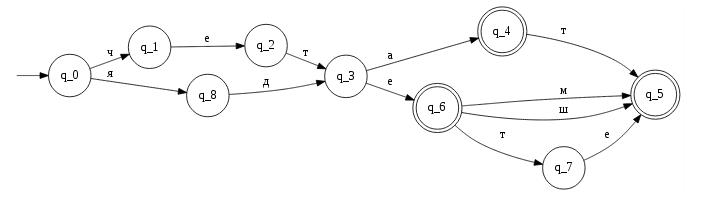
\includegraphics{figures/example2.jpg}
  \caption{Автомат, разпознаващ словоформите \textbf{\emph{яда}}, \textbf{\emph{ядеш}}, \textbf{\emph{яде}},
  \textbf{\emph{ядем}}, \textbf{\emph{ядете}}, \textbf{\emph{ядат}},
  \textbf{\emph{чета}}, \textbf{\emph{четеш}}, \textbf{\emph{чете}},
  \textbf{\emph{четем}}, \textbf{\emph{четете}}, \textbf{\emph{четат}}}
\end{figure}

  Фигура 1. визуализира автомата, който разпознава словоформите
  \textbf{\emph{ям}}, \textbf{\emph{ядеш}}, \textbf{\emph{яде}},
  \textbf{\emph{ядем}}, \textbf{\emph{ядете}}, \textbf{\emph{ядат}},
  \textbf{\emph{чета}}, \textbf{\emph{четеш}}, \textbf{\emph{чете}},
  \textbf{\emph{четем}}, \textbf{\emph{четете}}, \textbf{\emph{четат}}.
  Автоматът се състои от 11 състояния и 16 прехода.
  Фигура 2. визуализира автомата, който разпознава словоформите
  \textbf{\emph{яда}}, \textbf{\emph{ядеш}}, \textbf{\emph{яде}},
  \textbf{\emph{ядем}}, \textbf{\emph{ядете}}, \textbf{\emph{ядат}},
  \textbf{\emph{чета}}, \textbf{\emph{четеш}}, \textbf{\emph{чете}},
  \textbf{\emph{четем}}, \textbf{\emph{четете}}, \textbf{\emph{четат}}.
  Автоматът се състои от 9 състояния и 12 прехода. Този автомат се е получил, като сме премахнали словоформата \textbf{\emph{ям}} и сме я заменили със словоформата
  \textbf{\emph{яда}}. Това води до намаляване на размера на автомата с 2 състояния и 4 прехода.

\pagebreak

\section{Общи дефиниции и обозначения}

\begin{defn}
Ако $R \subseteq A_1 \times A_2 \times ... \times A_n$ е релация, то с $Proj_iR = \{a_i | (a_1...a_i...a_n) \in R\}$ означаваме i-тата прокеция на R.
\end{defn}

\begin{defn}
Ако $R$ е релация, с $R^+$ означаваме транзитивното затваряне на $R$.
\end{defn}

\begin{defn}
Азбука $\Sigma$ наричаме всяко крайно множество от символи.
\end{defn}

\begin{defn}
Казваме, че $\alpha$ е дума над азбуката $\Sigma$, ако $\alpha$ е крайна последователност от символи от $\Sigma$ и пишем $\alpha = a_1a_2...a_n$, $n \in \mathbb N$.
Дължината на $\alpha$ отбелязваме с $|\alpha|$. Ако $|\alpha| = n$, пишем още $\alpha \in \Sigma^n$.
С $\alpha_1$ отбелязваме $a_1$, с $\alpha_2$ - $a_2$, ..., с $\alpha_n$ - $a_n$.
\end{defn}

\begin{defn}
Ако $n, m \in \mathbb N$, $\alpha = a_1a_2...a_n \in \Sigma^n$, $\beta = b_1b_2...b_m \in \Sigma^m$, тогава думата
$\alpha . \beta = a_1a_2...a_n . b_1b_2...b_m = a_1a_2...a_nb_1b_2...b_m \in \Sigma^{n+m}$ наричаме конкатенация на думите $\alpha$ и $\beta$.
\end{defn}

\begin{defn}
Със $\varepsilon$ означаваме празната дума (с дължина 0).
\end{defn}

\begin{defn}
Множеството от всички думи над азбука $\Sigma$ бележим със $\Sigma^*$, където $\Sigma^* = \bigcup\limits_{n=0}^{\infty} \Sigma^n$.
\end{defn}

\begin{defn}
Език L над азбука $\Sigma$ наричаме всяко подмножество на $\Sigma^*$.
\end{defn}

\begin{defn}
Краен детерминиран автомат наричаме нареденната петторка $A = ( \Sigma, Q, s, F, \delta )$, където
$\Sigma$ е крайна азбука, Q е крайно множество от състояния, $s \in Q$ е началното състояние, $F \subseteq Q$ е множеството от финални състояния,
$\delta : Q \times \Sigma \pfun Q$ е частична функция на преходите.
\end{defn}

\begin{defn}
Път в крайния детерминиран автомат $A = ( \Sigma, Q, s, F, \delta )$ наричаме последователността от преходи
$((q_1, a_1), q_2), ((q_2, a_2), q_3), ..., ((q_n, a_n), q_{n+1})$, където за $\forall i \in \{1, 2, ..., n\} \;\delta(q_i, a_i)=q_{i+1}$.
Такъв път означаваме с $\pi: q_1 \xrightarrow{a_1} q_2 \xrightarrow{a_2} q_3 \xrightarrow{a_3} .... \xrightarrow{a_{n  - 1}} q_n \xrightarrow{a_n} q_{n+1}$.
$q_1$ наричаме начало на $\pi$, $q_{n + 1}$ - край на $\pi$, $a_1a_2...a_n$ - етикет на $\pi$, n - дължина на $\pi$.
\end{defn}

\begin{defn}
Крайният детерминиран автомат $A = ( \Sigma, Q, s, F, \delta )$ наричаме ацикличен, ако всеки път в А
$\pi: q_1 \xrightarrow{a_1} q_2 \xrightarrow{a_2} q_3 \xrightarrow{a_3} .... \xrightarrow{a_{n  - 1}} q_n \xrightarrow{a_n} q_{n+1}$
е такъв, че за $\forall i \in \{1, 2, ..., n+1\}$ $\forall j \in \{1, 2, ..., n+1\}$ $i \neq j$ $\implies$ $q_i \neq q_j$.
\end{defn}

\begin{defn}
Рефлексивното и транзитивно затваряне на $\delta$ е частичната функция $\delta^* : Q \times \Sigma^* \pfun Q $, която се дефинира по следния начин:
\begin{enumerate}
 \item[1)] $\delta^*(q, \varepsilon) = q$
 \item[2)] $\delta^*(q, a_1a_2...a_n) = \delta^*(\delta(q, a_1), a_2...a_n)$
\end{enumerate}
\end{defn}

\begin{stm}
Нека $A = (\Sigma, Q, s, F, \delta)$ е краен детерминиран автомат. \\$\delta^*(q_1, w) = q_n$ $\Leftrightarrow$ съществува път
$\pi: q_1 \xrightarrow{w_1} q_2 \xrightarrow{w_2} q_3 \xrightarrow{w_3} .... \xrightarrow{w_{|w| - 1}} q_{n - 1} \xrightarrow{w_{|w|}} q_n$.
\end{stm}

\begin{defn}
Нека $A = (\Sigma, Q, s, F, \delta)$ е краен детерминиран автомат и $q \in Q$. Тогава $\delta_q = \left.{\delta}\right|_{\{q\} \times \Sigma}$.
\end{defn}

\begin{defn}
Нека $A = (\Sigma, Q, s, F, \delta)$ е краен детерминиран автомат и $q \in Q$. Тогава множеството
$\vec{L}_A(q) = \{w \in \Sigma^* | \delta^*(q, w) \in F\}$ наричаме десен език на състоянието q в автомата A.
\end{defn}

\begin{defn}
Нека $A = (\Sigma, Q, s, F, \delta)$ е краен детерминиран автомат. Език на автомата А наричаме множеството
$L(A) = \vec{L}_A(s)$.
\end{defn}

\begin{defn}
Нека $A = (\Sigma, Q, s, F, \delta)$ е краен детерминиран автомат. Казваме, че състоянията $q_1$ и $q_2$ $\in Q$ са еквивалентни,
ако $\vec{L}_A(q_1) = \vec{L}_A(q_2)$.
\end{defn}

\begin{defn}
Нека $A = (\Sigma, Q_A, s_A, F_A, \delta_A)$ е краен детерминиран автомат. Казваме, че А е минимален, ако за всички
крайни детерминирани автомати $B = (\Sigma, Q_B, s_B, F_B, \delta_B)$, такива че L(A) = L(B), $|Q_A|\;\leq\;|Q_B|$.
\end{defn}

\begin{thm}
Минималният автомат A за даден език L е единствен с точност до изоморфизъм.
\end{thm}

\begin{defn}
Нека $A = (\Sigma, Q_A, s_A, F_A, \delta_A)$ е краен детерминиран автомат и $q \in Q_A$ е произволно състояние. $q$ наричаме достижимо, ако
$\exists w_1 \in \Sigma^* \; \delta_A(s_A, w_1) = q$.
\end{defn}

\begin{defn}
Нека $A = (\Sigma, Q_A, s_A, F_A, \delta_A)$ е краен детерминиран автомат и $q \in Q_A$ е произволно състояние. $q$ наричаме кодостижимо, ако
$\exists w_2 \in \Sigma^* \; \delta_A(q, w_2) \in F_A$.
\end{defn}

\begin{defn}
Нека $A = (\Sigma, Q_A, s_A, F_A, \delta_A)$ и $B = (\Sigma, Q_B, s_A, F_B, \delta_B)$ са крайни детерминирани
автомати. B = trim(A), ако $Q_B = \{q | q \in Q_A \;\&\; \exists w_1 \in \Sigma^* \; \delta_A(s_A, w_1) = q \;\&\; \exists w_2 \in \Sigma^* \; \delta_A(q, w_2) \in F_A\} $,
$\delta_B = \left.{\delta_A}\right|_{Q_B \times \Sigma}$ и $F_B = F_A \cap Q_B$.
\end{defn}

\begin{defn}
Нека $ A = ( \Sigma, Q, s, F, \delta )$ е краен детерминиран автомат. Обем на A наричаме числото $V(A)\;=\;|Q|\;+\;|dom(\delta)|$.
\end{defn}
\pagebreak

\section {Формално описание и решение на задачата}

  $\hspace*{5mm}$ Всеки естествен език е краен и може да се представи с минимален ацикличен детерминиран краен автомат $A = (\Sigma, Q_A, s_A, F_A, \delta_A)$.
  Целта на задачата е да намерим минимален ацикличен детерминиран краен автомат $\widehat{B}$, чийто език $L(\widehat{B})$ е максимално близък до езика $L(A)$ и същевременно
  $V(\widehat{B}) \le V(A)$. Така поставената задачата може да се разглежда като оптимизационна задача при подходяща целева функция и гранични условия.
  Нека $MADFSA = \{ B = (\Sigma, Q_B, s_B, F_B, \delta_B) \}$ е множеството от всички минимални ациклични детерминирани крайни автомати.
  Целевета функция, която искаме да опитимизираме е $F_A(B) : MADFSA \times MADFSA \fun \mathbb R$.
  Без ограничение на общността можем да считаме, че търсим максимум на целевата функция. Граничните условия, които поставяме са
  $g_j(B) \leq c_j ; B \in MADFSA; c_j \in \mathbb R; j \in \{1, ..., m\}$.
  Търсеният автомат ${\widehat{B}} = \argmax_B F_A(B)$.\\

  $\hspace*{5mm}$ Трябва да се пресметне $F_A(B)$ за всички автомати $B \in MADFSA$, за които $V(B) \le V(A)$ и
  $g_j(B) \leq c_j ; c_j \in \mathbb R; j \in \{1, ..., m\}$.
  Техният брой е не по-малко от експоненциален спрямо $V(A)$ и следователно при предположение, че сложността за пресмятане на целевата функция и
  на граничните условия е константа, сложносста на алгоритъма ще бъде също не по-малко от експоненциална спрямо $V(A)$.
  Следният пример демонстрира, че този брой в действителност е експоненциален спрямо $V(A)$.

  \begin{example}
  \hfill \break\ \hfill \break
  $ A = (\Sigma, Q_A, s_A, F_A, \delta_A) $ \\
  $ \Sigma = \{ a_1, a_2, ..., a_n \} $ \\
  $ Q_A = \{ q_0, q_1, .. q_n \} $ \\
  $ s_A = q_0 $ \\
  $ F_A = \{ q_1, .. q_n \} $ \\
  $ \delta_A = \{ ((q_0, a_i), q_i)\;|\;i \in \{ 1, 2, .. , n \} \} $ \\
  $ V(A) = |Q_A| + | dom(\delta_A) | = n + 1 + n = 2n + 1 $ \\
  \hfill \break\
  $ I \subseteq \{ 1, 2, .. , n \} $ \\
  $ B = ( \Sigma, Q_A, s_A, F_A, \{ ((q_0, a_i), q_i)\;|\;i \in I \} ) $ \\
  $ V(B) = n + 1 + |I| $ \\
  $ V(B) = n + 1 + |I| \leq n + 1 + |\{ 1, 2, .. , n \}| = n + 1 + n = 2n + 1 = V(A) $ \\
  \hfill \break\
  $ Z = \{ B | I \subset \{ 1, 2, .. , n \} \} $ \\
  $ |Z| = 2^n $ \\
  \hfill \break\
  $ Q' \subseteq Q $ \\
  $ C = ( \Sigma, Q', s_A, Q' \cap F, \left.{\delta_A}\right|_{Q' \times \Sigma} ) $ \\
  $ V(C) = |Q'| + |dom(\left.{\delta_A}\right|_{Q' \times \Sigma})| $ \\
  $ V(C) = |Q'| + |dom(\left.{\delta_A}\right|_{Q' \times \Sigma})| \leq |Q_A| + |dom(\delta_A)| = 2n + 1 = V(A) $ \\
  \hfill \break\
  $ Y = \{ C | Q' \subseteq Q \} $ \\
  $ |Y| = 2^{|Q|} = 2 ^ {n + 1} $ \\
  \hfill \break\
  $ |Z| + |Y| = 2^n + 2 ^ {n+1} $
  \end{example}

\bigskip

  В по-нататъшното изложение е предложен алчен алгоритъм със линейна сложност спрямо $V(A)$ за решение на задачата, който намира автомат $\widetilde{B}$,
  локален максимум на целевата функцията.

  Алгоритъмът построява итеративно крайна редица $B_0 \rightarrow B_1 \rightarrow ... \rightarrow B_n$, $n \in \mathbb N$, като
  $B_i \in MADFSA i in \{1, ..., n\}$ и $B_0 = A$.
  Всеки член на редицата $B_i$ получаваме от предходния $B_{i-1}$, като
  прилагаме краен брой операции, чрез които получаваме от $B_{i-1}$ нови крайни ациклични детерминирани автомати. Ако множеството от тези автомати означим с $C_i$,
  тогава $B_i = \argmax_{B \in C} F_A(B)$. Тъй като целевата функция зависи от обема на автомата, естествено е на всяка стъпка да разглеждаме минимални
  автомати, за които всички състояния са достижими и кодостижими. Алгоритъмът приключва, когато $V(B_i) \leq k$ или когато $F(B_{i-1}) > F(B_i)$, като
  $\widetilde{B} = B_n$ е търсеният локален максимум на функцията. Ясно е, че алгоритъмът ще приключи за краен брой стъпки, тъй като на всяка стъпка разглеждаме
  краен брой автомати, всеки от които е с краен брой състояния и преходи.

\bigskip
  В конкретната реализация на алгоритъма разглеждаме три операции, но преди да ги разгледаме ще дадем допълнително дефиниции за
  четири функции, които поддържаме за ефективната реализация на алгоритъма:

\bigskip
\begin{defn} Нека $A = (\Sigma, Q_A, s_A, F_A, \delta_A)$  е краен автомат. Тогава функцията $indeg : Q_A \fun \mathbb N$,
$indeg(q) = |\{(q_1, a) | ((q_1, a), q) \in \delta_A \}|$ наричаме полустепен на входа на състоянието q.
\end{defn}
\begin{defn} Нека $A = (\Sigma, Q_A, s_A, F_A, \delta_A)$  е краен автомат. Тогава функцията $outdeg : Q_A \fun \mathbb N$,
$outdeg(q) = |\{(a, q_1) | ((q, a), q_1) \in \delta_A \}|$ наричаме полустепен на изхода на състоянието q.
\end{defn}
\begin{defn} Нека $A = (\Sigma, Q_A, s_A, F_A, \delta_A)$  е краен ацикличен автомат. Тогава функцията  $height : Q_A \fun \mathbb N$,
$height(q) = max \{ |\alpha|\;|\;\alpha \in \vec{L_A}(q) \}$ e дължината на най-дългата дума в десния език на състоянието q.
\end{defn}
\begin{defn} Нека $A = (\Sigma, Q_A, s_A, F_A, \delta_A)$  е краен автомат. Тогава функцията $h : Q_A \fun \{0,1\} \times 2 ^{ \Sigma \times Q_A}$,
$h(q) = \{ (q \in F, \{(a, q_1) | ((q, a), q_1) \in \delta_A\}) \}$ наричаме хеш за състоянието q.
\end{defn}

\bigskip
 Трите операции, които разглеждаме са следните:

\begin{defn}\label{def2}
Нека $A = (\Sigma, Q_A, s_A, F_A, \delta_A)$  е краен детерминиран ацикличен автомат. Казваме, че крайният детерминиран ацикличен автомат B се получава от А
чрез изтриване на прехода $((q_1, a), q_2)$, ако $B = (\Sigma, Q_A, s_A, F_A, \delta_A \backslash \{((q_1, a), q_2)\})$. Записваме $B = delTr(A, ((q_1, a), q_2)). $ \\
\end{defn}

\begin{defn}\label{def3}
Нека $A = (\Sigma, Q_A, s_A, F_A, \delta_A)$  е краен детерминиран ацикличен автомат. Казваме, че крайният детерминиран ацикличен автомат B се получава от А
чрез добавяне на прехода $((q_1, a), q_2)$, ако $B = (\Sigma, Q_A, s_A, F_A, \delta_A \cup \{((q_1, a), q_2)\})$, $\neg !\delta_A(q_1, a)$ и
$\neg \exists w \in \Sigma^*\;(!{\delta_A}^*(q_2, w) \land {\delta_A}^*(q_2, w) = q_1)$ .\\ Записваме $B = addTr(A, ((q_1, a), q_2))$.
\end{defn}

\begin{defn}\label{def4}
Нека $A = (\Sigma, Q_A, s_A, F_A, \delta_A)$  е краен детерминиран автомат. Казваме, че крайният детерминиран автомат B се получава от А чрез добавяне на
дадено състояние $q \in Q_A$ към финалните състояния, ако $B = (\Sigma, Q_A, s_A, F_A \cup \{q\}, \delta_A)$ и $q \notin F_A$. Записваме
$B = fin(A, q).$ \\
\end{defn}

\bigskip

 Тогава на всяка стъпка разглеждаме следните множества от крайни детерминирани ациклични автомати:

\bigskip

\begin{itemize}
 \item $C_1 = \{min(trim(delTr(B_{i-1}, ((q_1, a), q_2))))|\forall ((q_1, a), q_2) \in \delta_{B_{i-1}} \}$.
 \item $C_2 = \{min(addTr(B_{i-1}, ((q_1, a), q_2))) |
     \forall q_1 \in Q_{B_{i-1}} \forall a \in \Sigma \forall q_2 \in Q_{B_{i-1}} :\\
         (\neg !\delta_{B_{i-1}}(q_1, a)) \land \\
         (\exists q_3 \in Q_{B_{i-1}}: \{ (b, \delta_{B_{i-1}}(q_1, b)) | b \in Sigma \land !\delta_{B_{i-1}}(q_1, b) \} \cup
           \{(a, q_2)\} = \\ \{ (b, \delta_{B_{i-1}}(q_3, b)) | b \in Sigma \land !\delta_{B_{i-1}}(q_3, b) \}) \land \\
         (\neg \exists w \in \Sigma^*\;(!{\delta_A}^*(q_2, w) \land {\delta_A}^*(q_2, w) = q_1)) \}$.
 \item $C_3 = \{min(fin(B_{i-1}, q_1))|\forall q_1 \in Q_{B_{i-1}} \backslash F_{B_{i-1}} \}$.
\end{itemize}

Автоматът $B_i = \argmax_{B \in C_1 \cup C_2 \cup C_3} F_A(B)$. 

\begin{defn}
Нека $A = (\Sigma, Q, s, F, \delta)$ е краен детерминиран автомат и $p \in Q$. Тогава $QL_A(p) = \{q \in Q \;|\; \exists w \in \Sigma^* \;\delta^*(q, w) = p\}$.
\end{defn}

\bigskip

Ясно е, че ако всички състояния на даден автомат са достижими и кодостижими, то при операциите добавяне на ребро и прибавяне на
финално състояние това свойство ще се запази. Интересен е случаят при изтриване на ребро. Тъй като от автомата изтриваме само едно ребро, е достатъчно да се
разгледат състоянията, които са предшественици на левия край на реброто и тези, които са наследници на десния край. Тогава
функцията $trim$ може да реализираме чрез две индукции. Полустепента на изхода на левия край на изтития преход намалява с единица.
Ако новата стойност е равна на 0, тогава изтриваме даденото състояние, всичките му входящи преходи и по индукция прилагаме същата
процедура за предшествениците му. Полустепента на входа на десния край на реборото намалява с единица. Ако новата стойност е равна на 0, тогава изтриваме
даденото състояние, всичките му изходящи преходи и по индукция прилагаме същата процедура за предшествениците му. За ефективната реализация използваме
функциите indeg и outdeg, за които вече са дадени дефиниции.

\bigskip

Функцията $min$ по даден краен детерминиран ацикличен автомат връща еквивалентен на него минимален автомат. И при трите разгледани операции
десните езици на част от състоянията остават непроменени. Променят се само десните езици на състоянията от $QL(q_1)$. Ясно е, че в най-лошият случай
$|QL(q_1)|$ може да е съизмеримо с $|Q|$. Правим предположение, което може да се провери емпирично, че за автоматите, които представляват естествени езици,
$|QL(q_1)|$ е значително по-малко от $|Q|$. Това предположение използваме съществено в алгоритъма за минимизиране. За всяко състояние сме сметнали предварително
дължината на най-дългата дума в десния му език. Подреждаме състоянията от $QL(q_1)$ по нарастваща стойност на тази дължина. За всяко от тях проверяваме има ли
еквивалентно нему състояние в останалата част от автомата $Q \backslash QL(q_1)$. Тази проверка правим за време $O(1)$, като използваме хеш функцията h,
за която вече дадохме дефиниция.
Ако няма еквивалентно състояние, тогава текущото състояние е част от минималния автомат. Ако има еквивалентно състояние, тогава можем да изтрием текущото
състояние и да пренасочим всичките му входящи предходи към еквивалентното състояние. Така общата сложност за минимизиране на автомата ще бъде $|QL(q_1)|$.
Следва твърдение и доказателство, че така предложеният алгоритъм за минимизация е коректен.

\begin{thm}
Нека $A = (\Sigma, Q_A, s_A, F_A, \delta_A)$ и $B = (\Sigma, Q_B, s_B, F_B, \delta_B)$ са крайни детерминирани автомати и B се получава от А чрез изтриване на
прозоволен преход $((q_1, a), q_2) \in \delta_A$. Тогава, ако $q \in Q_B$ е произволно състояние и $q \notin QL_A(q_1)$, то $\vec{L}_B(q) = \vec{L}_A(q)$.
\end{thm}

\begin{mproof}
Нека $((q_1, a), q_2) \in \delta_A$ е произволен и фиксиран преход в $A = (\Sigma, Q_A, s_A, F_A, \delta_A)$ и B се получава от А чрез изтриване на този преход, тоест
$B = (\Sigma, Q_A, s_A, F_A, \delta_A \backslash \{(q_1, a, q_2)\})$. Нека $q \in Q_B$
е произволно и фиксирано състояние, за което е в сила $q \notin QL_A(q_1)$.\\
$\hspace*{5mm}$Нека $w \in \vec{L}_B(q)$. Тогава в автомата B съществува път
$\pi: q = \xi_0 \xrightarrow{w_1} \xi_1 \xrightarrow{w_2} .... \xrightarrow{w_{|w|-1}} \xi_{|w|-1} \xrightarrow{w_{|w|}} \xi_{|w|},
\xi_{|w|} \in F_B$, но всеки път в B е път и в A. Следователно $\pi$ е път и в автомата А и $w \in \vec{L}_A(q)$.
Получихме, че за произволна дума $w \in \vec{L}_B(q)$, следва че $w \in \vec{L}_A(q)$.\\
$\hspace*{5mm}$Обратно, нека $w \in \vec{L}_A(q)$. Тогава в автомата А съществува път
$\pi: q = \xi_0 \xrightarrow{w_1} \xi_1 \xrightarrow{w_2} .... \xrightarrow{w_{|w|-1}} \xi_{|w|-1} \xrightarrow{w_{|w|}} \xi_{|w|}, \xi_{|w|} \in F_A$,
такъв че $\forall i \in \{0, 1,..., |w|\} \;\xi_i \neq q_1$. Ако допуснем, че за някое
$i \in \{0, 1,..., |w|\} \;\xi_i = q_1$, тогава получваме, че $\delta_A^*(q, w_1w_2...w_i) = \xi_i = q_1$ (в частност при i = 0 имаме, че
$\delta_A^*(q, \varepsilon) = q = \xi_0 = q_1$), тоест $q \in QL_A(q_1)$, което е в противоречие с условието.
Следователно всеки преход $((\xi_i, w_{i+1}, \xi_{i+1})$ е различен от прехода $((q_1, a), q_2)$, но тогава $\pi$ е път и в B.
Следователно $w \in \vec{L}_B(q)$. Получихме, че за произволна дума $w \in \vec{L}_A(q)$, следва че $w \in \vec{L}_A(B)$.\\
$\hspace*{5mm}$Окончателно получаваме, че за произволна дума w, $w \in \vec{L}_A(q)$ т.с.т.к $w \in \vec{L}_A(B)$. Следователно $\vec{L}_B(q) = \vec{L}_A(q)$.
\end{mproof}

\begin{thm}
Нека $A = (\Sigma, Q_A, s_A, F_A, \delta_A)$ и $B = (\Sigma, Q_B, s_B, F_B, \delta_B)$ са крайни детерминирани ациклични автомати и B се получава от А чрез
добавяне на преход $((q_1, a), q_2)$, като $\neg !\delta_A(q_1, a)$ и $\neg \exists w \in \Sigma^*: \; \pi : q_2 \xRightarrow{w} q_1$ е път в A.
Тогава, ако $q \in Q_B$ е произволно състояние и $q \notin QL_B(q_1)$, то $\vec{L}_B(q) = \vec{L}_A(q)$.
\end{thm}

\begin{mproof}
Нека $A = (\Sigma, Q_A, s_A, F_A, \delta_A)$ и B се получава от А чрез добавяне на преход $((q_1, a), q_2)$, като
$\neg !\delta_A(q_1, a)$ и $\neg \exists w \in \Sigma^*: \; \pi : q_2 \xRightarrow{w} q_1$ е път в A.
Тоест $B = (\Sigma, Q_A, s_A, F_A, \delta_A \cup \{(q_1, a, q_2)\}$. Нека $q \in Q_B$ е произволно и фиксирано състояние, за което е в сила
$q \notin QL_B(q_1)$.\\
$\hspace*{5mm}$Нека $w \in \vec{L}_A(q)$. Тогава в автомата A съществува път
$\pi: q = \xi_0 \xrightarrow{w_1} \xi_1 \xrightarrow{w_2} .... \xrightarrow{w_{|w|-1}} \xi_{|w|-1} \xrightarrow{w_{|w|}} \xi_{|w|},
\xi_{|w|} \in F_A$, но всеки път в A е път и в B. Следователно $\pi$ е път и в автомата B и $w \in \vec{L}_B(q)$.
Получихме, че за произволна дума $w \in \vec{L}_A(q)$, следва че $w \in \vec{L}_B(q)$.\\
$\hspace*{5mm}$Обратно, нека $w \in \vec{L}_B(q)$. Тогава в автомата B съществува път
$\pi: q = \xi_0 \xrightarrow{w_1} \xi_1 \xrightarrow{w_2} .... \xrightarrow{w_{|w|-1}} \xi_{|w|-1} \xrightarrow{w_{|w|}} \xi_{|w|}, \xi_{|w|} \in F_B$,
такъв че $\forall i \in \{0, 1,..., |w|\} \;\xi_i \neq q_1$. Ако допуснем, че за някое
$i \in \{0, 1,..., |w|\} \;\xi_i = q_1$, тогава получваме, че $\delta_B^*(q, w_1w_2...w_i) = \xi_i = q_1$ (в частност при i = 0 имаме, че
$\delta_B^*(q, \varepsilon) = q = \xi_0 = q_1$), тоест $q \in QL_B(q_1)$, което е в противоречие с условието.
Следователно всеки преход $((\xi_i, w_{i+1}, \xi_{i+1})$ е различен от прехода $((q_1, a), q_2)$, но тогава $\pi$ е път и в A.
Следователно $w \in \vec{L}_A(q)$. Получихме, че за произволна дума $w \in \vec{L}_B(q)$, следва че $w \in \vec{L}_A(B)$.\\
$\hspace*{5mm}$Окончателно получаваме, че за произволна дума w, $w \in \vec{L}_A(q)$ т.с.т.к $w \in \vec{L}_A(B)$. Следователно $\vec{L}_B(q) = \vec{L}_A(q)$.
\end{mproof}

\begin{lemma}
Нека $A = (\Sigma, Q_A, s_A, F_A, \delta_A)$ е детерминиран краен минимален ацикличен автомат, $B = (\Sigma, Q_B, s_B, F_B, \delta_B)$ е краен детерминиран
ацикличен автомат и B се получава от А чрез изтриване или добавяне на преход $((q_1, a), q_2)$. Тогава в $Q_B \backslash QL(q_1)$ няма различни еквивалентни
състояния.
\end{lemma}

\begin{mproof}
Да допуснем, че $r, t \in Q_B \backslash QL(q_1)$ и r и t са еквивалентни състояния в автомата B, тоест $\vec{L}_B(r) = \vec{L}_B(t)$,
но $r, t \notin QL(q_1)$ и следователно $\vec{L}_A(r) = \vec{L}_B(r) = \vec{L}_B(t) = \vec{L}_A(t)$. Това означава, че r и t са екввалентни състояния и в
автомата A, което е в противоречие с това, че A е минимален. Следователно r и t не са еквивалентни състояния в автомата B.
\end{mproof}

\begin{thm}
Нека $A = (\Sigma, Q_A, s_A, F_A, \delta_A)$ е детерминиран краен минимален ацикличен автомат, $B = (\Sigma, Q_B, s_B, F_B, \delta_B)$ е краен детерминиран
ацикличен автомат и B се получава от А чрез изтриване или добавяне на преход $((q_1, a), q_2)$. Тогава предложеният алгоритъм за минимизация е коректен.
\end{thm}

\begin{mproof}
Нека $r_1, r_2, .. r_p$ са всички състояния от $QL(q_1)$, сортирани по нарастваща дължина на най-дългата дума в десния им език. Ще докажем, че ако на стъпка i
състоянието $r_i$ има еквивалентно нему състояние t, то $Proj_1{\delta_t} = Proj_1{\delta_{r_i}}$. Наистина нека допуснем, че $r_i$ и t са еквивалентни, но
$Proj_1{\delta_t} \neq Proj_1{\delta_{r_i}}$. Тогава съществува $w \in \vec{L}_B(r_i) = \vec{L}_B(t)$, такова че
$\delta(r_i, w1) = p_1 \neq \delta(t, w1) = p_2$. Но $p_1$ и $p_2$ са еквивалентни. Ако допуснем, че $p_1$ и $p_2$ не са еквивалентни, тогава
$\vec{L}(p_1) \neq \vec{L}(p_2)$. Нека тогава $\alpha \in \vec{L}(p_1)$, но $\alpha \notin \vec{L}(p_2)$. Но тогава думата $w_1\alpha \in \vec{L}(r_i)$ и
$w_1\alpha \notin \vec{L}(t)$, което е противоречие с това, че $r_i$ и t са еквивалентни. Аналогичен е случаят
$\alpha \notin \vec{L}(p_1)$, но $\alpha \in \vec{L}(p_2)$. Следователно получаваме, че $p_1$ и $p_2$ са еквивалентни. От лема [3.1] е ясно, че не може и двете
състояния $p_1$ и $p_2$ да бъдят в $Q_B \backslash QL(q_1)$. Тогава нека без ограниечение на общността $p_1 \in QL(q_1)$. Тъй като $p_1$ и $p_2$ са еквивалентни,
следва че $p_1$ е по-надясно в редицата $r_1, r_2, .. r_p$ от $r_i$. Нека $\beta = max \{|\gamma| | \gamma in \vec{L}(p_1)\} $, но тогава
$|w1\beta| > |\beta|$ и $|w1\beta| \in \vec{L}(r_i)$, което е противоречие с това, че състоянията са сортирани по нарастваща дължина на най-дългата дума в 
десния им език. Случаят $p_2 \in QL(q_2)$ е аналогичен. Противоречието идва от допускането, че $Proj_1{\delta_t} \neq Proj_1{\delta_{r_i}}$. Следователно
$Proj_1{\delta_t} = Proj_1{\delta_{r_i}}$. След стъпка p автоматът ще е минимален.
\end{mproof}

\pagebreak

\section{Резултати}

\begin{center}
  \begin{table}[h]\label{tableResults}
    \centering
    \begin{tabular}{|c||c|c|c|c|c|c|}\hline
            & $V(A)$ & $V(B)$ & \%    & $|L(B) \setminus L(A)|$ & $|L(A) \setminus L(B)|$ & Брой итерации \\\hline
    \end{tabular}
    \caption{Резултати}
  \end{table}
\end{center}

\pagebreak

\section{Заключение}

\pagebreak

\begin{thebibliography}{}

\bibitem{citation01}
\newblock Derrick G. Kourie, Bruce W. Watson, Loek Cleophas, and Fritz Venter.
\newblock Failure Deterministic Finite Automata

\bibitem{citation02}
\newblock Henrik Björklund, Johanna Björklund, Niklas Zechner.
\newblock Compression of finite-state automata through failure transitions

\bibitem{citation03}
\newblock Kalin Georgiev.
\newblock Compression of minimal acyclic deterministic FSAs preserving the linear accepting complexity

\bibitem{citation04}
\newblock Jan Daciuk and Jakub Piskorski.
\newblock Gazetteer Compression Technique Based on Substructure Recognition

\bibitem{citation05}
\newblock Руселина Ницолова.
\newblock Българска граматика. Морфология.
\newblock 2008

\end{thebibliography}

\end{document}
